\documentclass[11pt]{article}

\usepackage{acl}
\usepackage{times}
\usepackage{latexsym}
\usepackage{microtype}
\usepackage{inconsolata}
\usepackage{graphicx}
\usepackage{booktabs}
\usepackage{amsmath}
\usepackage{url}
\usepackage{xspace}

\newcommand{\ergm}{ERGM\xspace}

\title{FORGE: An LLM-Assisted System for Proposing and Testing Explanations of Network Tie Formation}

\author{Yidan Sun \\
  University of Southern California \\
  \texttt{yidans@usc.edu} \\\And
  Mayank Kejriwal \\
  Information Sciences Institute, \\
  University of Southern California \\
  \texttt{kejriwal@isi.edu}}

\hypersetup{
  pdftitle={FORGE: An LLM-Assisted System for Proposing and Testing Explanations of Network Tie Formation},
  pdfauthor={Yidan Sun, Mayank Kejriwal}
}

\begin{document}
\maketitle

\begin{abstract}

Networks are ubiquitous, from friendships in schools and collaborations among scientists to trade between organizations, and a long-standing question is why ties form. Exponential Random Graph Models (ERGMs) let researchers test possible explanations, but specifying a useful model is hard: informal ideas such as ``similar actors connect'' must be translated into valid statistical terms, combined into a stable formula, and checked against the observed network. Large language models (LLMs) can suggest explanations, but unconstrained outputs may include invalid terms, unstable models, or claims unsupported by the fitted results. We present FORGE, an interactive system that turns a user-supplied network and a short description of its setting into checked candidate explanations of tie formation. The LLM proposes formulas restricted to terms valid for the input network and writes the final plain-language account; code and statistical checks decide what is accepted. Across twelve benchmark networks, FORGE attained the lowest BIC in 9 of 10 converged comparisons. The demo and source package are available at \url{https://yidans.github.io/forge-demo/}.

\end{abstract}


\section{Introduction}
\label{sec:introduction}

\begin{figure*}[t]
\centering
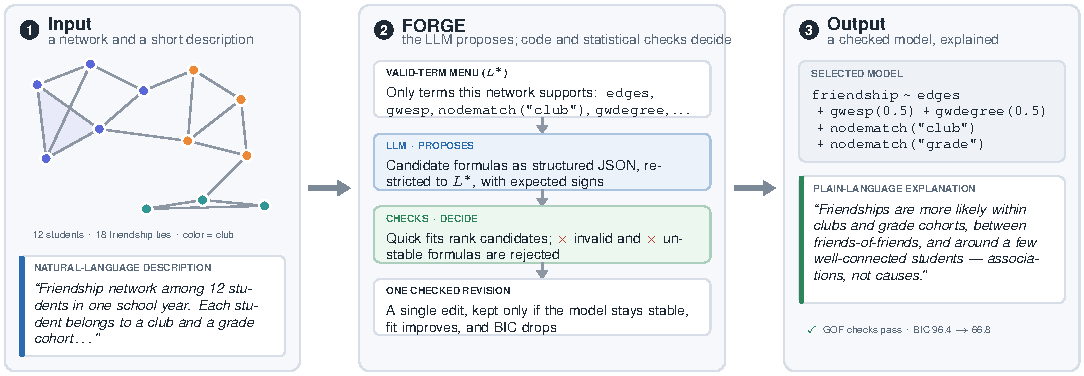
\includegraphics[width=0.98\linewidth]{fig1_pipeline.pdf}
\caption{\textbf{FORGE at a glance.} From a user-supplied network and a short natural-language description (left), FORGE builds the menu of ERGM terms valid for that network, asks an LLM to propose candidate formulas restricted to that menu, screens the candidates with statistical checks, and permits one checked revision (middle). The output is a selected model together with a plain-language, non-causal explanation of which ideas about tie formation it supports (right). All values shown come from the school-friendship run walked through in Section~\ref{sec:interface}. Throughout, the LLM proposes formulas and explanations, while code and statistical checks decide what is accepted.}
\label{fig:forge-overview}
\end{figure*}

\begin{figure*}[!t]
    \centering
    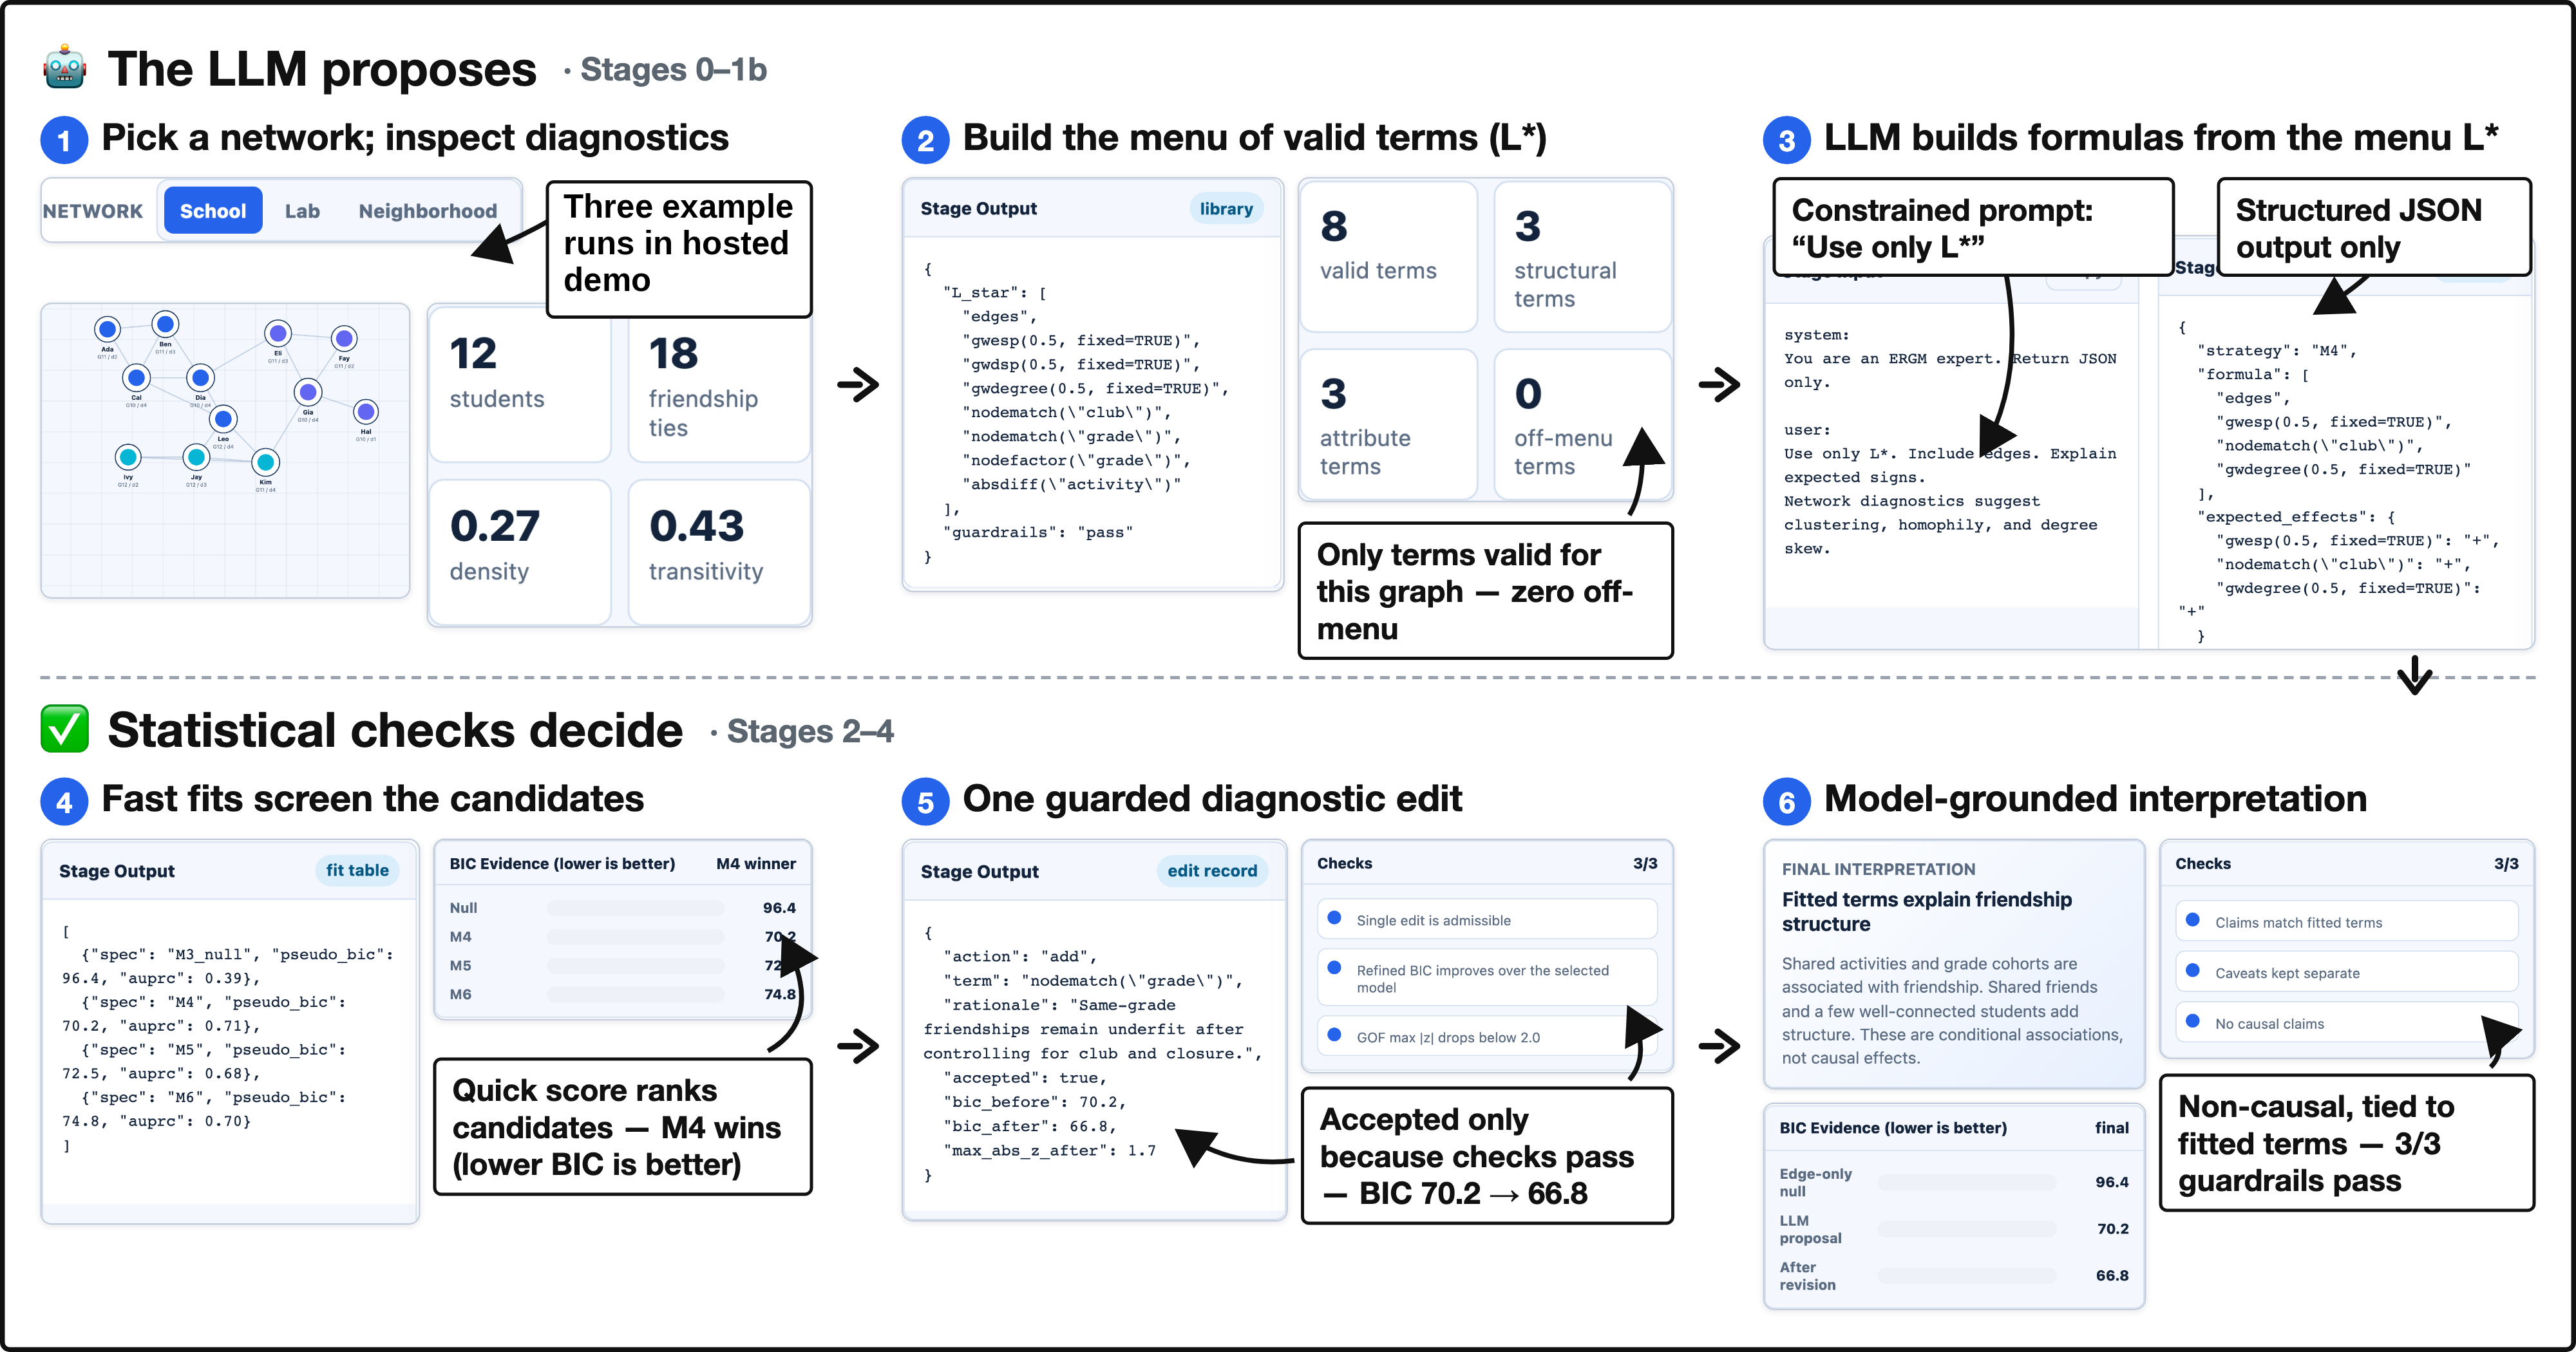
\includegraphics[width=0.91\textwidth]{interface_v3.png}
    \caption{\textbf{Browser walkthrough for one completed school-friendship record.} Top row: the user inspects the input network (1); FORGE builds the list of model terms available for that network, $L^{*}$ (2); and the LLM returns candidate formulas as structured JSON using only terms from $L^{*}$ (3). Bottom row: quick fits rank the candidates (4); one proposed revision is accepted only after it passes the checks and improves fit (5); and the final model is explained in plain language without causal claims (6). The hosted interface contains three bundled records, while the released local pipeline accepts new networks through the documented input format and presents their stages in the same browser view.}
    \label{fig:interface}
\end{figure*}

Networks are ubiquitous, from friendships in schools and collaborations among scientists to trade between organizations \citep{newman2003structure,borgatti2009network}. A long-standing question in network science is why ties form: why two students become friends, why two researchers co-author, or why one organization trades with another. Over the past three decades, one family of models has become a standard way to answer such questions: Exponential Random Graph Models (ERGMs) \citep{wasserman1996logit,robins2007introduction,lusher2013ergm}. An ERGM looks much like a regression over a whole network: each term expresses one idea about why ties form, such as homophily (similar actors form ties), triadic closure (a friend of a friend becomes a friend), or degree heterogeneity (a few actors attract many ties), and fitting the model estimates how strongly each idea is associated with the observed ties. Much of the appeal of ERGMs is that they combine these ideas in a single equation; in addition, they come with well-understood statistical machinery for estimation and checking. Figure~\ref{fig:forge-overview} (right) shows an example of such a model.

The hard part is writing that equation. Given a network and a short natural-language description of its setting, choosing and combining terms remains an ad hoc, trial-and-error process that depends on the analyst's experience and habits: some terms do not apply to the network at hand, some combinations make estimation unstable \citep{schweinberger2011instability}, and a fitted model may still reproduce the observed network poorly, so analysts typically go through several rounds of revision and refitting.

For NLP researchers, ERGM specification brings together two familiar tasks. The first is to turn a plain-language description into a valid structured output. The second is to explain a fitted result without going beyond what the evidence supports. In this setting, the system must translate a short description of the network into an ERGM formula built from a restricted list of valid terms, and then explain the fitted model using only the relationships supported by the results. LLMs can help propose possible reasons why ties form \citep{yao2023react,schick2023toolformer}. On their own, however, they may use terms that do not apply to the network, propose models that cannot be fit reliably, or make claims stronger than the fitted results allow. FORGE therefore splits the work: the LLM proposes candidate explanations and writes summaries, while code and statistical checks decide what is accepted.

FORGE helps users generate and test possible explanations for why ties form in a network. A user provides the network, any available attributes attached to nodes or pairs, and a short natural-language description of the setting. FORGE then asks the LLM to suggest possible explanations, such as ties being reciprocated, actors connecting through shared contacts, similar actors connecting, or a small number of actors receiving many ties. The system translates these ideas into ERGM formulas that are valid for the input network. It removes formulas that fail basic checks or cannot be fit reliably, compares the remaining candidates, and allows one checked revision. The final output explains, in plain language, which proposed explanations are included in the selected model, as associations consistent with the observed network. Figure~\ref{fig:forge-overview} summarizes this workflow on a school friendship network.

FORGE includes an executable R pipeline and a browser interface. The R pipeline processes a network, calls the LLM, fits the candidate models, and applies the checks. The browser presents each step, including the network, the prompt sent to the LLM, the returned response, the fit results, and the reason each candidate was accepted or rejected (Figure~\ref{fig:interface}). The hosted demonstration replays three bundled stage records rather than making new API calls or fitting new models. The same repository provides the local server and R code needed to run the workflow on a new network and present its stages in the browser. This keeps the hosted demonstration reliable and fast without implying that the static site is a compute service.

Key contributions include:
\begin{itemize}
\item We present a workflow that turns a user-supplied network and a short domain description into competing explanations of tie formation, represented as ERGM formulas that are valid for the input.
\item We implement an executable R pipeline that proposes, fits, checks, and explains candidate models, together with a browser interface that makes every proposal and decision visible.
\item We release the runnable local pipeline, its documented network input format, and three browser records containing the stage prompts, responses, statistical summaries, and acceptance decisions shown in the hosted walkthrough.
\end{itemize}


\begin{table*}[t]
\centering
\small
\begin{tabular}{@{}p{0.12\linewidth}p{0.26\linewidth}p{0.26\linewidth}p{0.24\linewidth}@{}}
\toprule
Stage & What FORGE does & What the user sees & Acceptance rule \\
\midrule
0. Intake & Load a network, its attributes, and basic summaries. & Network view, density, transitivity, and degree summaries. & Reject inputs with missing attributes, self-loops, or unsupported graph types. \\
1a. Valid terms & List the ERGM terms available for the input network. & Term list with plain-language labels. & Filter by tie direction, available attributes, and term support. \\
1b. LLM proposals & Turn possible explanations into candidate formulas. & JSON formulas and expected directions. & Reject unavailable terms and malformed output. \\
2. Fit and select & Screen candidates with fast approximate fits and approximate BIC. & Candidate ranking and selected model. & Require the baseline term, prefer a simpler formula when fit is similar, and improve on the edge-only baseline. \\
3. Revision & Use fit checks to request one small change. & Accepted or rejected change. & Accept only valid, stable changes that improve the fit checks and BIC. \\
4. Explanation & Explain which ideas about tie formation appear in the fitted model. & Plain-language explanation with evidence and limits. & Tie each claim to a fitted term and avoid causal language. \\
\bottomrule
\end{tabular}
\caption{The R pipeline produces each stage result, and the browser shows that result together with the rule used to accept or reject it. The LLM proposes formulas and explanations; code and statistical checks make the final decisions.}
\label{tab:stages}
\end{table*}

\section{System Overview}
\label{sec:system}
FORGE has two components: an R pipeline that runs the analysis and a browser client that lets users inspect the result. The pipeline accepts a network $G=(V,E,X)$ and an optional natural-language description, builds the list of ERGM terms available for that network, calls the LLM, screens and fits candidate formulas, and allows at most one checked revision. The local server converts these outputs into the stage structure shown by the browser: the term list, LLM requests and responses, fit results, revision decision, and final explanation. Table~\ref{tab:stages} summarizes the stages.

\paragraph{User-supplied inputs.}
The pipeline is not limited to the three networks in the hosted interface. A user provides an edge list, whether ties are directed, optional node or pair-level attributes, and a short description of the setting. FORGE checks the input and builds only the terms supported by that network. The current release handles binary directed and undirected networks and the attribute types included in its term list. During a local run, the server presents the outputs using the same stage structure as the hosted browser.

\paragraph{Saved runs and browser view.}
The browser's stage record contains the input network, node and pair-level attributes, network summaries, the valid ERGM term list, LLM requests and responses, candidate formulas, screening results, fit summaries, revision decisions, and the final explanation. The hosted records are bundled with the static client, so the stage rail, graph view, prompt and response panels, and evidence sidebar require no external service calls during a presentation. In local mode, the browser builds the same structure from the local server's outputs.

\paragraph{Stage 0: network intake.}
The workflow begins with the input network. Users see the nodes, ties, attributes, and basic summaries, including density, transitivity, degree summaries, and validity checks. These facts guide the later prompts and determine which model terms are available.

\paragraph{Stage 1: valid terms and candidate explanations.}
FORGE first builds a graph-specific list of ERGM terms (denoted $L^{*}$): the terms that can be used for the input network. Terms for reciprocated ties appear only for directed networks, and attribute terms appear only when the required node or pair-level attribute is present. The LLM then proposes possible explanations of tie formation and expresses them as JSON formulas drawn from this list. Users can see whether every proposed term is available for the network.

\paragraph{Stage 2: candidate screening.}
FORGE ranks the candidate formulas before the slower final fit. It scores each candidate with a fast approximate fit (maximum pseudo-likelihood), removes candidates that do not improve on a baseline containing only the overall tie rate, and flags clear signs of instability. Users see the ranking, the selected model, and the numbers behind that choice.

\paragraph{Stage 3: diagnostic revision.}
The selected formula is then tested with goodness-of-fit (GOF) summaries, which compare networks simulated from the fitted model with the observed network. When these checks show a clear miss, the LLM may propose one small edit, such as adding, removing, or replacing a term. The edit is accepted only if it uses valid terms, remains stable, improves the GOF checks, and lowers the Bayesian information criterion (BIC). The browser shows both the proposed edit and the decision.

\paragraph{Stage 4: checked plain-language explanation.}
The final stage keeps the model fixed and explains which ideas about tie formation appear in the fitted result. Users see the final terms, fit evidence, passing checks, and graph views that link the explanation to visible parts of the network. The prompt tells the LLM to avoid causal claims and to keep supported findings separate from limits, so the text explains the fitted model rather than adding a new result.

\section{User Interface}
\label{sec:interface}

FORGE includes a browser client for interactive inspection of the pipeline stages. The hosted client operates in replay mode and reads three bundled example records. It does not issue new LLM calls or fit ERGMs during the session. The locally served client can instead call the released Python and R workflow. Figure~\ref{fig:interface} walks through one bundled record and shows where the LLM proposes, where the checks decide, and what evidence supports each accepted result.

\paragraph{Intended audience and demonstration script.}
The system is designed for two audiences. NLP researchers see a complete example of constrained generation with external verification: the LLM returns structured proposals, and statistical checks decide which are accepted. Network analysts see how LLM assistance fits into a standard \texttt{ergm}-style workflow while the fitting, screening, and accept/reject decisions stay with the statistical machinery. A typical live demonstration takes two to three minutes: the presenter walks one run from Stage 0 to Stage 4, then switches to a second network to show the same pipeline selecting a different explanation for a different graph.

\paragraph{Example runs.}
The hosted interface includes three small completed scenario records selected for quick inspection:
\begin{itemize}
    \item \textbf{School friendship}: tests shared activities, grade cohorts, common friends, and highly connected students as possible explanations of friendship ties.
    \item \textbf{Research collaboration}: tests shared areas, similar roles, common collaborators, and bridge researchers as possible explanations of collaboration ties.
    \item \textbf{Neighborhood mutual aid}: tests same-block proximity, shared neighbors, helper hubs, and similar residence history as possible explanations of help ties.
\end{itemize}
Each run has its own attributes, edges, term list, candidate formulas, revision record, and final explanation. Switching examples resets the interface to Stage 0, so the presenter can repeat the full walkthrough during a live session.

\paragraph{Prompt and output transparency.}
The lower panels show the input prompt and structured output for the active stage. For example, Stage 1b shows the specification request and the JSON formula proposal (a compact example is reproduced in Appendix~\ref{app:record}), while Stage 3 shows the revision request and the accepted or rejected edit record. This makes the LLM step easy to check, and makes FORGE visibly different from a black-box chatbot: each LLM step has a constrained input, a structured output the system can check, and a visible accept/reject decision.

\paragraph{Visual explanation.}
The graph view changes as users move through the stages. For homophily terms, it marks ties within a group; for closure terms, it marks triangle-like structures; and in the final view, it marks the nodes and ties linked to the accepted model. These visual cues connect ERGM terms such as \texttt{gwesp(0.5)} to visible features of the network.

\paragraph{Example walkthrough.}
In the school friendship scenario, Stage 0 loads 12 students with 18 undirected ties and reports density 0.27 and transitivity 0.43. Stage 1a builds an eight-term list, combining structural terms such as \texttt{gwesp}, \texttt{gwdsp}, and \texttt{gwdegree} with attribute terms supported by the available node attributes. Stage 1b shows JSON formulas restricted to this list; the selected candidate combines a baseline \texttt{edges} term with triadic closure, club homophily, and degree heterogeneity. Stage 2 ranks the candidates with fast approximate fits and selects this formula, reducing the approximate BIC from 96.4 to 70.2. Stage 3 shows a revision that adds \texttt{nodematch("grade")}; the edit passes the checks, improves BIC to 66.8, and is logged as accepted. Stage 4 presents the fitted terms as a short, non-causal explanation in which friendship ties are associated with shared contexts and shared friends. The bundled record exposes the formulas, numerical summaries, checks, and decisions shown in this walkthrough; new local runs expose the same stage structure.


\section{System Validation and End-to-End Evaluation}
\label{sec:evaluation}
We evaluate FORGE at two levels. First, we test whether the browser reliably displays and links the result from each stage. Second, we ask whether the executable pipeline can start from a benchmark network and select a valid, well-fitting explanation under the same fitting settings.

\paragraph{Interface validation.}
We tested the browser interface in desktop viewports. The checks cover the main actions used during a short presentation: selecting each of the three networks, resetting to Stage 0 after a network switch, moving from Stage 0 to Stage 4, updating the final interpretation and ERGM terms for each network, showing non-empty graph views, and running without console errors.

\paragraph{End-to-end pipeline evaluation.}
We tested FORGE on twelve benchmark networks, including school friendship, workplace and organizational ties, email communication, covert networks, and Facebook social networks. For each network, the system received only the observed ties, the available node or pair-level attributes, and a short description of the setting. It was not given a final ERGM formula written by an expert. We compared FORGE against random term selection (Random-K), an edge-only null model, and LLM-only variants that propose formulas without FORGE's screening and revision checks. All methods used the same inputs, generated the same number of candidate models, and followed the same fitting settings. After the initial screening step, every surviving candidate was refit with Monte Carlo maximum likelihood estimation (MCMLE), and we compared the fitted models using BIC.

\begin{figure}[t]
\centering

\includegraphics[width=0.86\columnwidth]{baseline_improvement.pdf}
\caption{\textbf{Pipeline comparison on converged benchmark networks.} Bars show mean BIC improvement over the edge-only null for the ten networks where non-null full ERGM refits converged; error bars show 95\% Student-$t$ confidence intervals, and dots show individual networks. Axis labels report how often each method attained the lowest BIC.}
\label{fig:baselines}
\end{figure}

Figure~\ref{fig:baselines} summarizes the aggregate comparison. FORGE produced converged refits on 10 of 12 networks. On the two largest networks, no non-null candidate method converged under these settings, although the edge-only null fit did. Among the ten converged cases, FORGE achieved the lowest BIC in 9 cases and improved null BIC by 26.4\% on average, compared with 23.1\% for the best LLM-only baseline. This comparison measures fit and model-selection quality across networks; it does not show that the selected explanation is causal or uniquely true.

\section{Related Work}
\label{sec:related}

\paragraph{ERGM specification.}
ERGMs formalize hypotheses about network tie formation as exponential-family statistics over graphs \citep{wasserman1996logit,robins2007introduction}. The \texttt{statnet} and \texttt{ergm} ecosystems provide widely used tools for fitting, simulation, and diagnostics \citep{handcock2008statnet,hunter2008ergm,krivitsky2023ergm4}. Even with these tools, specification remains difficult because some terms and term combinations can lead to degeneracy or poor mixing \citep{schweinberger2011instability}. FORGE builds on this statistical toolchain but focuses on a different part of the workflow: helping users move from their own network and a short domain description to a set of checked candidate explanations.

\paragraph{Constrained and structured LLM outputs.}
A long-standing problem in NLP is turning natural language into valid executable forms, such as logical forms or SQL queries \citep{berant2013semantic,yu2018spider}. Prior work has shown that generation can be constrained by a target grammar or schema, for example through incremental parsing during decoding \citep{scholak2021picard}. FORGE uses a similar idea for statistical model building. Rather than letting the LLM write arbitrary formulas, the system gives it a graph-specific ERGM term library, asks for a parseable specification, and checks each candidate before fitting.

\paragraph{LLMs for scientific workflows.}
LLMs are increasingly used in research workflows to suggest hypotheses, summarize evidence, and call external tools. Tool-use and reasoning/action frameworks show how language models can work with external APIs or environments instead of acting as standalone predictors \citep{yao2023react,schick2023toolformer}. FORGE takes a conservative version of this approach. The LLM suggests possible explanations of why ties form and writes the final plain-language account, but it does not estimate parameters, decide on its own whether a model fits well enough, or create terms outside the displayed list.

\paragraph{Interactive NLP systems.}
NLP system demonstrations often make intermediate states visible to users, from open model tooling \citep{wolf2020transformers} to interactive model-analysis interfaces such as the Language Interpretability Tool \citep{tenney2020lit}. FORGE brings this style of interaction to statistical network analysis. The browser interface is part of the contribution: it shows the input graph, LLM prompt, structured output, system checks, model evidence, and final interpretation in one step-by-step view.


\section{Conclusion}
\label{sec:conclusion}

We presented FORGE, an interactive network theory discovery assistant that turns a user-supplied network and a short domain description into checked candidate explanations of why ties form. The R pipeline proposes possible explanations, represents them as valid ERGM formulas, rejects weak or unstable candidates, and reports the explanations linked to the best checked model. The browser makes the prompts, fit evidence, and accept/reject decisions visible. The hosted interface presents three bundled scenario records, while the released local pipeline supports new networks through the documented input format. FORGE does not identify causal processes from an observed network; it helps analysts propose, compare, and inspect plausible explanations under explicit statistical checks. The demo and source package are publicly available under the MIT License.

\section*{Limitations}
\label{sec:limitations}
FORGE can only propose explanations that its term list can express. Mechanisms with no corresponding ERGM term in the current list are invisible to the system, and the system does not warn users about explanations it cannot represent. The current release also handles only binary directed and undirected networks, so ideas that require valued, longitudinal, or bipartite data cannot be tested. The quality and coverage of the candidates depend on the LLM. We evaluated a single model with fixed prompts, and its proposals may favor well-known mechanisms over less common ones; we did not measure sensitivity to prompt wording or model choice. Acceptance decisions likewise depend on the specific criteria we chose: the GOF summaries, the BIC comparison, and the single-revision budget. Different criteria or a larger revision budget could select different models, and the lowest-BIC candidate is only the best of the proposed set, not a guarantee of good absolute fit. On the two largest benchmark networks, no non-null candidate converged under our fixed fitting settings, so scaling to larger networks may require adaptive settings or longer runs. 

\section*{Ethics Statement}
\label{sec:ethics}

FORGE is intended to help analysts state the assumptions behind a network model. This can make the analysis easier to inspect, but it also creates risks if users over-interpret fitted terms, apply the system to sensitive networks, or treat LLM-generated explanations as causal evidence. The interface therefore shows the fit checks, states the limits, and avoids causal language. For domains such as security intelligence or workplace communication, users should ensure that data collection, analysis, and downstream decisions comply with applicable legal, institutional, and privacy requirements.


\section*{Availability and License}
\label{sec:availability}

FORGE is publicly available under the MIT License: the live demo at \url{https://yidans.github.io/forge-demo/} and the source package at \url{https://github.com/yidans/forge-demo}. The package includes the documented input format and local-run instructions for processing a new network.

\bibliography{references}

\appendix

\section{Example LLM Request and Response}
\label{app:record}
Figure~\ref{fig:record} shows the compact Stage 1b request and response displayed for the school example in the browser.

% TODO before submission: replace this compact display with the exact full request
% sent to the model, including the expanded L*, JSON schema, exact model ID,
% and decoding settings. Keep the raw response unchanged.
\begin{figure}[ht]
\centering
\small
\begin{verbatim}
system:
You are an ERGM expert. Return JSON only.

user:
Use only L*. Include edges.
Explain expected signs.
Network diagnostics suggest clustering,
homophily, and degree skew.

{
  "strategy": "M4",
  "formula": [
    "edges",
    "gwesp(0.5, fixed=TRUE)",
    "nodematch(\"club\")",
    "gwdegree(0.5, fixed=TRUE)"
  ],
  "expected_effects": {
    "gwesp(0.5, fixed=TRUE)": "+",
    "nodematch(\"club\")": "+",
    "gwdegree(0.5, fixed=TRUE)": "+"
  }
}
\end{verbatim}
\caption{The compact Stage 1b request and structured JSON response shown for the school example in the browser.}
\label{fig:record}
\end{figure}

\end{document}
